\documentclass[12pt,a4paper]{article}
\usepackage[utf8]{inputenc}
\usepackage[russian]{babel}
\usepackage[left=2.00cm, right=2.00cm, top=2.00cm, bottom=2.00cm]{geometry}
\linespread{1.25}
\usepackage{setspace}
\usepackage{indentfirst}
\setlength{\parindent}{1.25cm}
\let\paragraph\ignorespaces
\usepackage{tabularx}
\usepackage{multirow}
\usepackage{graphicx}
\usepackage[Large]{titlesec}


\usepackage{graphicx}
\graphicspath{ {images/} }


\begin{document}
	
\begin{titlepage}
	
\begin{center}
	\large Университет ИТМО\\[5cm]
	\LARGE Практическая работа №1\\
	\normalsize по дисциплине <<Визуализация и моделирование>>\\[5cm]
\end{center}
\begin{flushright}
		\begin{minipage}{0.6\textwidth}
		\begin{flushleft}
			\large
			\singlespacing 
			\textbf{Автор:} Кумпан Виктор Викторович\\
			\textbf{Поток:} 1.2\\
			\textbf{Группа:} K3241\\
			\textbf{Факультет:} ИКТ\\
			\textbf{Преподаватель:} Чернышева А.В.
		\end{flushleft}
	\end{minipage}
\end{flushright}

\vfill

\begin{center}
	{\large Санкт-Петербург, \the\year{ г.}}
\end{center}
 
\end{titlepage}


\begin{center}
    \textbf{\Large{Аннотация}}
\end{center}

\large Описание датасета, состоящего из 7 акций американских компаний следующих секторов: IT, нефтегазового и фэшн индустрии. Формулировка глобальных задач, которые можно решить на данном датасете.

\section{Подбор датасета}

\large На протяжении года я занимаюсь инвестициями в акции американских компаний и мне интересно работать с такого рода данными. Информацию по акциям компаний взял с сайта investing.com. При выборе датасета я руководствовался следующим:


\begin{minipage}{0.9\textwidth}
			\large
			\singlespacing 
            \begin{itemize}
            \item \normalsize Выбор информации из сферы, которая мне интересна, и имеет для меня потенциал в развитии;
            \item \normalsize Пригодность этой информации к визуализации и моделированию;
            \item \normalsize Открытый доступ к информации;
            \item \normalsize Наличие примеров моделирование и визуализации данной информации в интернете, что свидетельствует о ее применимости к анализу.
            \end{itemize}
\end{minipage}

\section{Описание датасета}

\large Датасет состоит из акций 7 крупнейших американских компаний разных секторов за период 22.02.2018 - 22.02.2021, а именно:

\begin{minipage}{0.9\textwidth}
			\large
			\singlespacing 
            \begin{itemize}
            \item \normalsize Apple, IBM, Dell (IT сектор)
            \item \normalsize ExxxonMobil, Chevron Corp (Нефтяная добыча)
            \item \normalsize Nike,PVH Corp (Фэшн индустрия)
            \end{itemize}
\end{minipage}\\[0.25cm]


\large По каждой из акций информация представлена в виде .CSV файла следующей формы.

\newpage

\begin{center}
    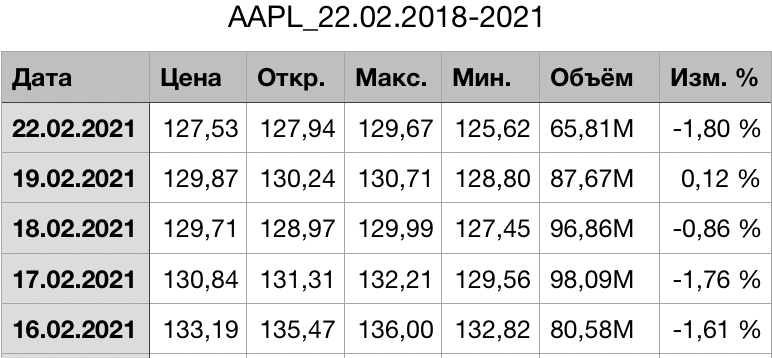
\includegraphics[width=0.5\textwidth]{StockApple.png}
\end{center}

\begin{figure}[h]
    \centering
    \caption{Пример данных по акции Apple}
    \label{fig:Stock1}
\end{figure}

\large На рисунке \ref{fig:Stock1} приведен пример датасета по ежедневным изменениям акций Apple, аналогичными критериями выборки обладают остальные 5 акции. В столбце "Цена" указана ежедневная стоимость одной акции во время закрытия торгов, стоимости установлены в \$. В остальных столбцах по аналогии, основываясь на их названии.

\large \textit {Почему был выбран датасет именно в таком сочетании акций?}

\large Идея выбора такого портфеля для анализа заключается в том, что с ним можно проводить различные виды анализа так, как он в какой-то мере диверсифицирован и имеет преобладающий сектор (IT). В таком случае мы можем составлять различные модели и визуализировать их в разных плоскостях.

\section{Глобальные задачи, решаемые на данном датасете}

\large Используя данный датасет мы можем решить следующие задачи:

\begin{minipage}{0.9\textwidth}
			\large
			\singlespacing 
            \begin{itemize}
            \item \normalsize Прогнозирование падения и роста акций;
            \item \normalsize Анализ стоимости акций IT сектора от внешнеполитических и прочих факторов;
            \item \normalsize Корреляция между активами IT сектора и другими не смежными секторами;
            \item \normalsize Анализ и визуализация рисков портфеля, в зависимости от внешнеполитических факторов;
            \item \normalsize Визуализация темпов развития различных секторов экономики США
            \end{itemize}
\end{minipage}\\[0.25cm]


\end{document}